The interaction of ultra-high intensity (UHI) lasers with solid matter at laser
pulse durations of few ten to hundred femtoseconds opens up the possibility to
study transient, non-equilibrium high energy density plasma processes on time
scales close to that of atomic processes with X-Ray free electron lasers with
nanometer resolution \cite{Kluge2016}.

\begin{figure}
\centering
  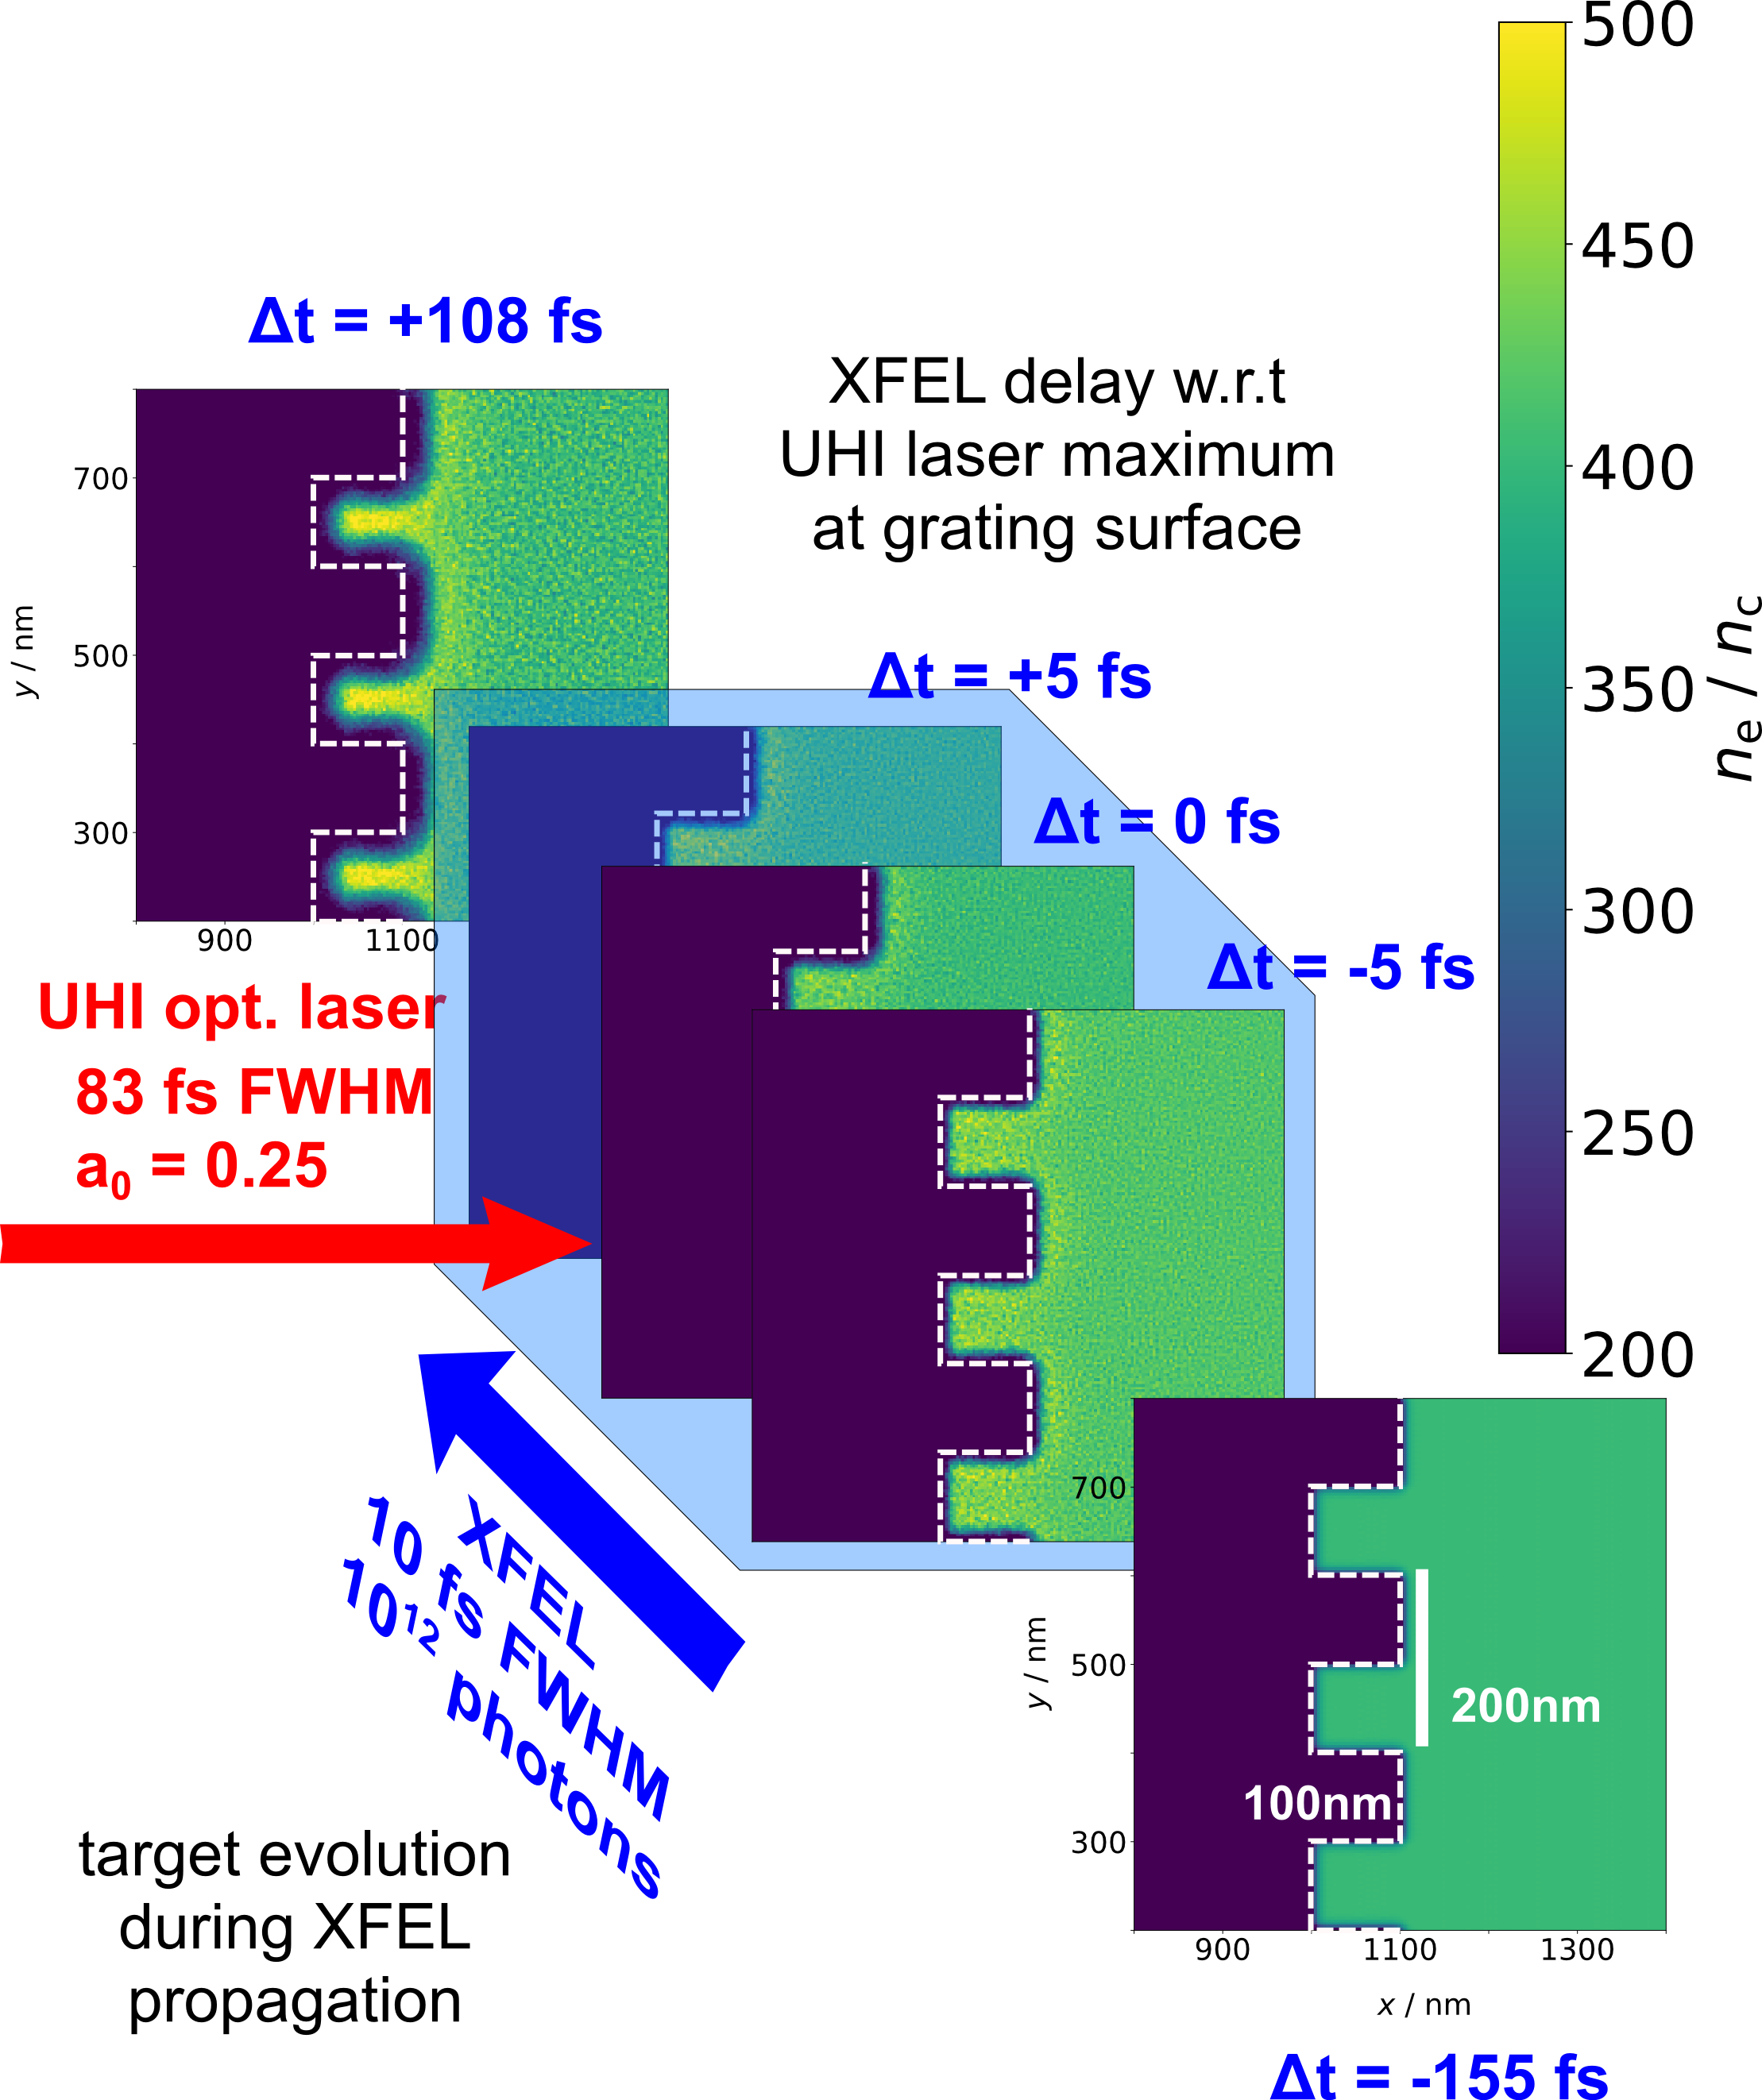
\includegraphics[width=.95\linewidth]{figures/scattering_geometry_v4.png}
\caption{
Scattering geometry with XFEL pulse perpendicular to optical UHI laser. The
target is a silicon foil with a grating surface. As the XFEL pulse traverses the
target, the electron density changes due to the UHI laser interacting with the
grating which dissolves over time. Delay times of the XFEL pulse maximum are
given with respect to the time when the optical laser pulse maximum hits the
target surface.  The area illuminated by the XFEL pulse is
$2\lambda_\mathrm{opt} \times 2\lambda_\mathrm{opt}$, with the corresponding
SAXS image, assuming $3\,\mathrm{µm}$ target depth, seen in Fig.
\ref{fig:scattering}.  }
  \label{fig:density}
\end{figure}

\begin{figure}
\centering
  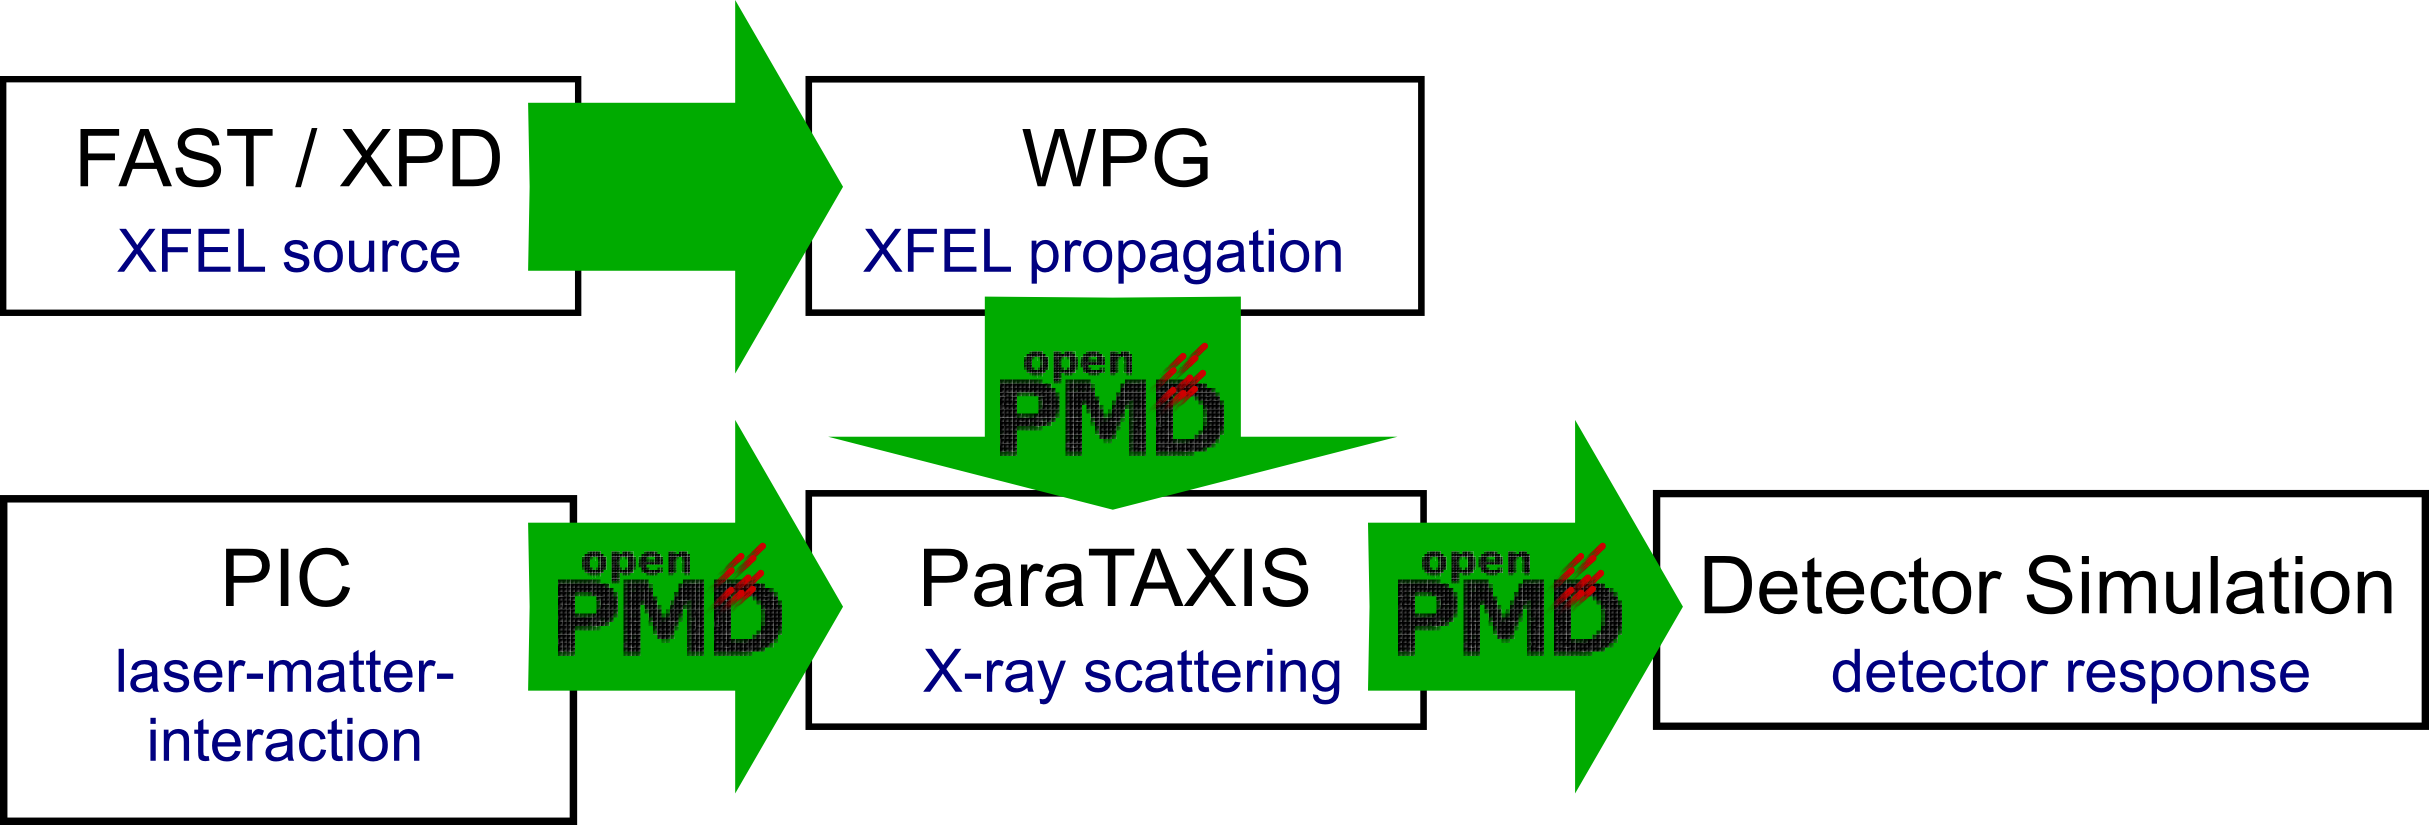
\includegraphics[width=.85\linewidth]{figures/simex_workflow_v2.png}
\caption{
SIMEX workflow connecting the simulation codes via data exchange in openPMD standard.
}
  \label{fig:workflows}
\end{figure}

Thus, radiation transport calculations must take these time and length scales
into account. We here introduce the example of softening and expansion of a
grating structure, see Fig. \ref{fig:density},  that is irradiated by an UHI
optical laser pulse to illustrate the possibilities of ParaTAXIS, a tool
developed within WP4 that resolves radiation transport on the single photon
level. ParaTAXIS is fully integrated into the simex\_platform tool chain via
openPMD \cite{Huebl2017} in- and output, see Fig. \ref{fig:workflows}.

We study a $\tau_\mathrm{opt} = 83\,\mathrm{fs}$ (FWHM), $\lambda_\mathrm{opt} =
0.8\,\mathrm{\mu m}$ laser pulse impinging on a silicon foil under 0° incidence
that drives the grating into a heated plasma state. An X-ray pulse of
$\tau_\mathrm{XFEL} = 10\,\mathrm{fs}$ (FWHM) with photon energy
$E_\mathrm{XFEL} =8.4\,\mathrm{keV}$ probes the surface grating structure
perpendicularly to the optical laser propagation with a delay relative to its
pulse maximum arriving at the target surface. With growing delay we expect the
scattering maxima of the grating to vanish as its edges soften and the plasma
expands into the vacuum.

The time structure of the XFEL pulse, the evolution of the target while the
pulse probes it and effects like multiple-scattering smear out the scattering
maxima. All effects are taken into account by ParaTAXIS. For SIMEX milestone 4.3
we present the interoperability of XFEL and UHI laser pulse generation,
interaction with the target and generation of a small-angle X-Ray scattering
(SAXS) image.

A particle-in-cell (PIC) simulation (milestone 4.2.2.7) provides the time
evolution of the electron density on which the XFEL photons are scattered. We
assume invariance of the target in propagation direction and simulate the XFEL
pulse with $10^{12}$ photons for which the setup is optically thin (milestone
4.2.2.9), see left part of Fig. \ref{fig:scattering}. We further demonstrate
scattering on an optically thick setup (milestone 4.2.2.10) by simulating
resonant scattering on the ions of the target. The ion density follows the
electron density as expected for plasma expansion into vacuum\cite{Mora2003},
see right part of Fig. \ref{fig:scattering}.

As expected, the signal of the optically thick target is washed out due to
higher scattering probability. In both, the optically thin and thick case the
SAXS pattern well resolves the nanometer-scale grating depth and period, taking
into account the target evolution during the interaction time with the laser
pulse.

All density data from the PIC simulation as well as the SAXS patterns are
published on Zenodo together with the data format documentation
\cite{Garten2017}.

\begin{figure}
\centering
  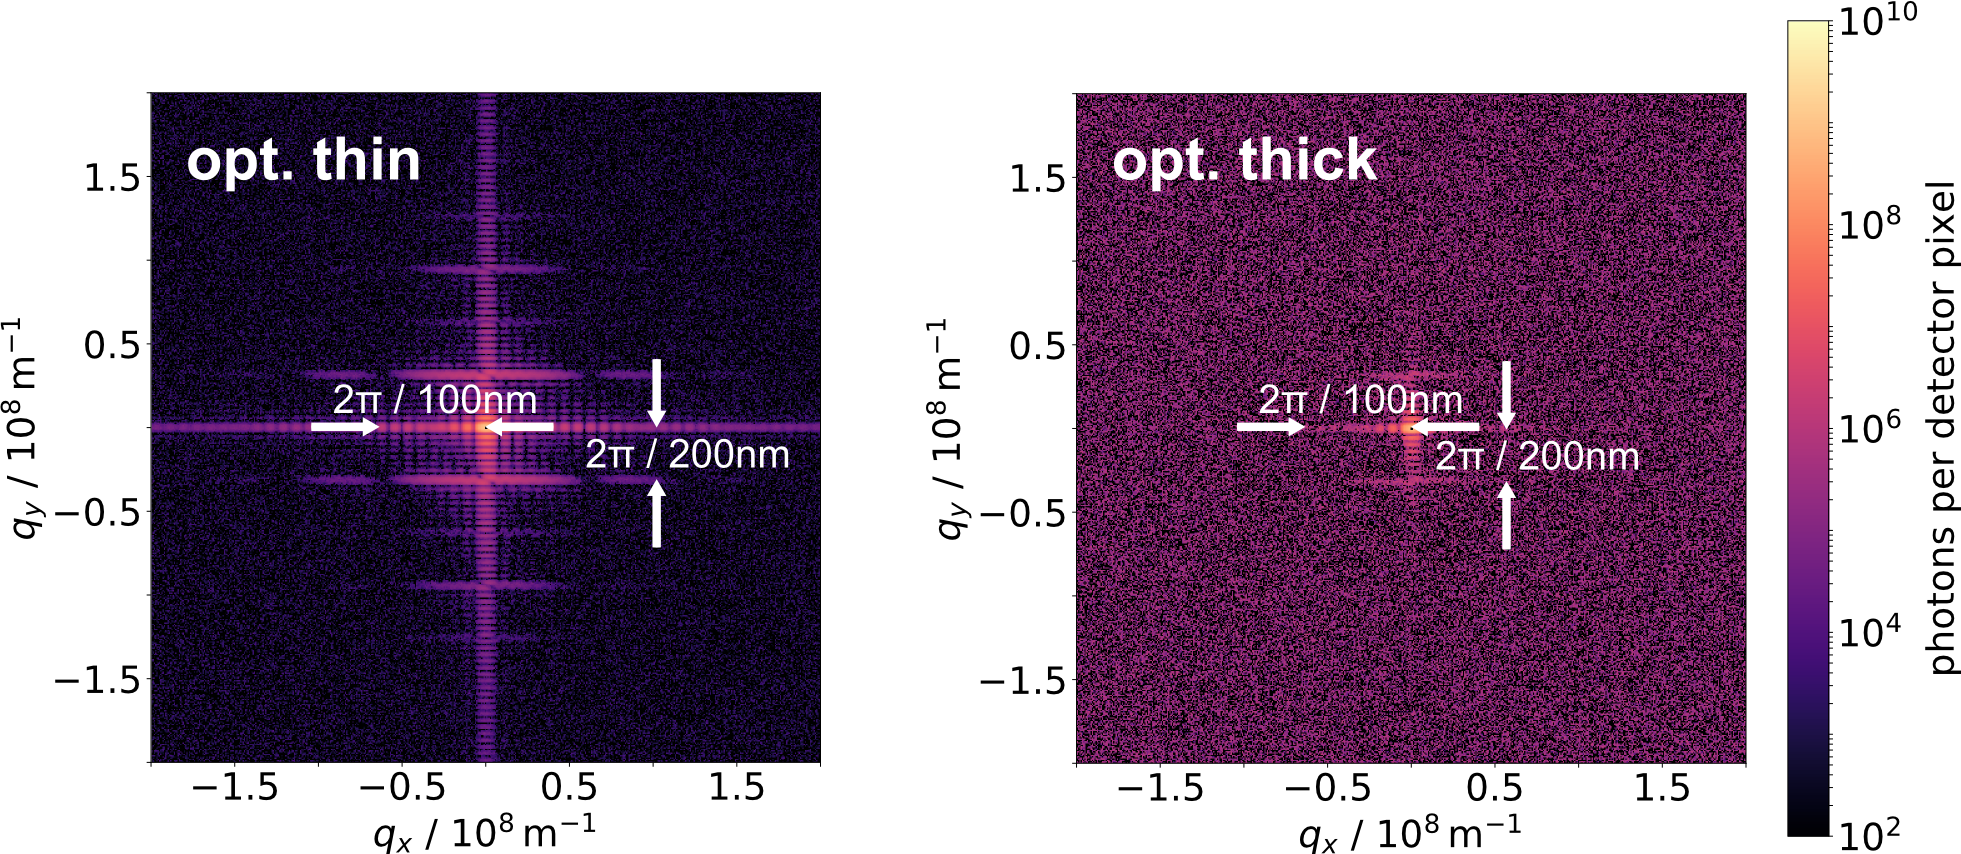
\includegraphics[width=.99\linewidth]{figures/scattering_images_v2.png}
\caption{
\textbf{Left:} ParaTAXIS SAXS image for the optically thin target at
$1.4\,\mathrm{m}$ distance from the target, detector pixel size $a_D =
13.5\,\mathrm{\mu m}$, X-ray wavelength $\lambda_\mathrm{XFEL} = 1.47\,$\AA\ and
$10^{12}$ photons in the illuminated area. The vertical separation of scattering
lines corresponds to the grating period of $200\,\mathrm{nm}$, the horizontal to
the grating depth of $100\,\mathrm{nm}$.
\textbf{Right:} ParaTAXIS SAXS image for the optically thick target. Here, the
scattering cross section was increased by a factor of 1000 to account for
resonant scattering at the ion density. All other parameters remain the same.  }
  \label{fig:scattering}
\end{figure}



